%% LyX 2.2.1 created this file.  For more info, see http://www.lyx.org/.
%% Do not edit unless you  know what you are doing.
\documentclass{article}\usepackage[]{graphicx}\usepackage[]{color}
% maxwidth is the original width if it is less than linewidth
% otherwise use linewidth (to make sure the graphics do not exceed the margin)
\makeatletter
\def\maxwidth{ %
  \ifdim\Gin@nat@width>\linewidth
    \linewidth
  \else
    \Gin@nat@width
  \fi
}
\makeatother

\definecolor{fgcolor}{rgb}{0.345, 0.345, 0.345}
\newcommand{\hlnum}[1]{\textcolor[rgb]{0.686,0.059,0.569}{#1}}%
\newcommand{\hlstr}[1]{\textcolor[rgb]{0.192,0.494,0.8}{#1}}%
\newcommand{\hlcom}[1]{\textcolor[rgb]{0.678,0.584,0.686}{\textit{#1}}}%
\newcommand{\hlopt}[1]{\textcolor[rgb]{0,0,0}{#1}}%
\newcommand{\hlstd}[1]{\textcolor[rgb]{0.345,0.345,0.345}{#1}}%
\newcommand{\hlkwa}[1]{\textcolor[rgb]{0.161,0.373,0.58}{\textbf{#1}}}%
\newcommand{\hlkwb}[1]{\textcolor[rgb]{0.69,0.353,0.396}{#1}}%
\newcommand{\hlkwc}[1]{\textcolor[rgb]{0.333,0.667,0.333}{#1}}%
\newcommand{\hlkwd}[1]{\textcolor[rgb]{0.737,0.353,0.396}{\textbf{#1}}}%
\let\hlipl\hlkwb

\usepackage{framed}
\makeatletter
\newenvironment{kframe}{%
 \def\at@end@of@kframe{}%
 \ifinner\ifhmode%
  \def\at@end@of@kframe{\end{minipage}}%
  \begin{minipage}{\columnwidth}%
 \fi\fi%
 \def\FrameCommand##1{\hskip\@totalleftmargin \hskip-\fboxsep
 \colorbox{shadecolor}{##1}\hskip-\fboxsep
     % There is no \\@totalrightmargin, so:
     \hskip-\linewidth \hskip-\@totalleftmargin \hskip\columnwidth}%
 \MakeFramed {\advance\hsize-\width
   \@totalleftmargin\z@ \linewidth\hsize
   \@setminipage}}%
 {\par\unskip\endMakeFramed%
 \at@end@of@kframe}
\makeatother

\definecolor{shadecolor}{rgb}{.97, .97, .97}
\definecolor{messagecolor}{rgb}{0, 0, 0}
\definecolor{warningcolor}{rgb}{1, 0, 1}
\definecolor{errorcolor}{rgb}{1, 0, 0}
\newenvironment{knitrout}{}{} % an empty environment to be redefined in TeX

\usepackage{alltt}
\usepackage[sc]{mathpazo}
\usepackage[T1]{fontenc}
\usepackage[english]{babel}
\usepackage[utf8]{inputenc}
\usepackage{geometry}
\usepackage{dsfont}
\usepackage{indentfirst}
\usepackage{fancyhdr}
\usepackage{amsmath}

% Margins of the document
\geometry{verbose,tmargin=2.5cm,bmargin=2.5cm,lmargin=2.5cm,rmargin=2.5cm}

% Header and footer for all pages
\pagestyle{fancy}
\fancyhf{}
\renewcommand{\headrulewidth}{0pt}
\rfoot{Page \thepage}

% Header and footer for first page
\fancypagestyle{plain}{%
  \renewcommand{\headrulewidth}{0pt}%
  \fancyhf{}%
  \rhead{ETH Zurich}
  \lhead{Applied Generalized Linear Models \\ Spring Semester 2020}
  \rfoot{Page \thepage}
}

%% Global Settings



\DeclareMathOperator{\SSR}{SSR}
\DeclareMathOperator{\SSreg}{SSreg}
\DeclareMathOperator{\SST}{SST}


%% ---------- BEGIN DOCUMENT -----------------------------------------------
\IfFileExists{upquote.sty}{\usepackage{upquote}}{}
\begin{document}

%% Tiltle
\title{Assignment 1}
\author{Milan Kuzmanovic, Mark McMahon \\ Martin Kotuliak, Jakub Polak}
\date{\today}

\maketitle

\section*{Task 1}

A multiple linear regression model has been estimated to study the relation- ship between $Y =$ violent crime rate (per 100,000 people), $X_1 =$ poverty rate (percentage with income below the poverty line) and $X_2 =$ percentage living in urban area. Data are collected in 51 cities in the U.S.\\

The relevant equations that relate estimate, standard error, T-statistic, R-squared and Sum of Squares of residuals, regression and total are folloqwing.

\[ \frac{\beta_i}{se(\beta_i)} = T_i \qquad R^2 = \frac{\SSreg}{\SST}= 1-\frac{\SSR}{\SST}  \qquad \SST = \SSreg + \SSR
\]

Using these we just plug in the corresponding information that is already provided and compute the missing values.

\begin{knitrout}
\definecolor{shadecolor}{rgb}{0.969, 0.969, 0.969}\color{fgcolor}\begin{kframe}
\begin{alltt}
\hlstd{a} \hlkwb{<-} \hlopt{-}\hlnum{498.683} \hlopt{/} \hlnum{140.988}
\hlstd{b} \hlkwb{<-} \hlnum{4.885} \hlopt{*} \hlnum{6.677}
\hlstd{c} \hlkwb{<-} \hlnum{9.112} \hlopt{/} \hlnum{6.900}
\hlstd{d} \hlkwb{<-} \hlnum{1841257.15} \hlopt{/} \hlstd{(}\hlnum{1} \hlopt{-} \hlnum{0.5708}\hlstd{)}
\hlstd{e} \hlkwb{<-} \hlstd{d} \hlopt{-} \hlnum{1841257.15}
\end{alltt}
\end{kframe}
\end{knitrout}

The table below reports the output with filled in missing information.

\begin{center}
\begin{tabular}{ l r r r r }
 \hline
            & Est.            & s.e.              & t-value         & p-value \\
 \hline
 Intercept  & -498.683  & 140.988 & $^{a\;}$-3.537 & 0.009 \\
 $X_1$      & $^{b\;}$32.617 & 6.677  & 4.885     & 0.001 \\
 $X_2$      & 9.112  & $^{c\;}$1.321 & 6.900      & 0.001 \\
 \hline
 $R^2$      & 0.5708            & & & \\
 SSreg      & $^{e\;}$2448718 & & & \\
 SSR        & 1841257.15        & & & \\
 SSTotal    & $^{d\;}$4289975 & & & \\
 \hline
\end{tabular}
\end{center}

The the coefficient of determination $R^2$ is $0.5708$. This value measures the proportion of the variance in $Y$ explained by the model. Hence, 57.08 \% of the sample variability of $Y$ can be explained by the linear combination of $X_i$'S given the sample data.\\

To compute the overall F-test we use the equation below and the statistic then follows an F distribution with corresponding degrees of freedom.
\[ F = \frac{\SSreg/p}{\SSR/(n-(p+1))} \sim F_{p,n-(p+1)}
\]

The data are collected in 51 cities, so $n=51$ and we have 2 predictors, so $p=2$. Other values we can easily obtain from the filled table above.
\begin{knitrout}
\definecolor{shadecolor}{rgb}{0.969, 0.969, 0.969}\color{fgcolor}\begin{kframe}
\begin{alltt}
\hlstd{(f} \hlkwb{=} \hlstd{(e} \hlopt{/} \hlnum{2}\hlstd{)} \hlopt{/} \hlstd{(}\hlnum{181257.15} \hlopt{/} \hlstd{(}\hlnum{51}\hlopt{-}\hlstd{(}\hlnum{2}\hlopt{+}\hlnum{1}\hlstd{)) ))}
\end{alltt}
\begin{verbatim}
## [1] 324.2312
\end{verbatim}
\end{kframe}
\end{knitrout}

Hence, the F-statistic has a value of 324.2311914. To interpret this, the global F-test, tests a null hypothesis that all regression coefficients are simultaneously 0. In a mathematical notation $H_0 : \beta_1 = \beta_2 = 0$. To evaluate the test, we can compute its p-value. It is a quantile of the corresponding F-distribution for the given statistic or mass under the distribution.

\begin{knitrout}
\definecolor{shadecolor}{rgb}{0.969, 0.969, 0.969}\color{fgcolor}\begin{kframe}
\begin{alltt}
\hlstd{(p} \hlkwb{=} \hlkwd{pf}\hlstd{(f,}\hlnum{2}\hlstd{,}\hlnum{48}\hlstd{,}\hlkwc{lower.tail} \hlstd{=} \hlnum{FALSE}\hlstd{))}
\end{alltt}
\begin{verbatim}
## [1] 1.319003e-28
\end{verbatim}
\end{kframe}
\end{knitrout}

The p-value is \ensuremath{1.3190029\times 10^{-28}}, which is very low and therefore there is a significant evidence against the null hypothesis that all regression coefficients are simultaneously zero. Hence, the p-value of a given sample is small and it suggests that the model with all the covariates is better than the one with just intercept coefficient. This test therefore determines if the linear model is at least suitable to explain some of the variance in the outcome variable. Which in this case it does.

\section*{Task 2}

\section*{Task 3}

\section*{Task 4}

\section*{Task Template}

This is just an expample of how to use latex and r-code chunks in knitr.\\

You can test if \textbf{knitr} works with this minimal demo. OK, let's
get started with some boring random numbers:

\begin{knitrout}
\definecolor{shadecolor}{rgb}{0.969, 0.969, 0.969}\color{fgcolor}\begin{kframe}
\begin{alltt}
\hlkwd{set.seed}\hlstd{(}\hlnum{1121}\hlstd{)}
\hlstd{(x}\hlkwb{=}\hlkwd{rnorm}\hlstd{(}\hlnum{20}\hlstd{))}
\end{alltt}
\begin{verbatim}
##  [1]  0.1449583  0.4383221  0.1531912  1.0849426  1.9995449 -0.8118832  0.1602680
##  [8]  0.5858923  0.3600880 -0.0253084  0.1508809  0.1100824  1.3596812 -0.3269946
## [15] -0.7163819  1.8097690  0.5084011 -0.5274603  0.1327188 -0.1559430
\end{verbatim}
\begin{alltt}
\hlkwd{mean}\hlstd{(x);}\hlkwd{var}\hlstd{(x)}
\end{alltt}
\begin{verbatim}
## [1] 0.3217385
## [1] 0.5714534
\end{verbatim}
\end{kframe}
\end{knitrout}

The first element of \texttt{x} is 0.1449583. Boring boxplots
and histograms recorded by the PDF device:

\begin{knitrout}
\definecolor{shadecolor}{rgb}{0.969, 0.969, 0.969}\color{fgcolor}\begin{kframe}
\begin{alltt}
\hlkwd{par}\hlstd{(}\hlkwc{mar}\hlstd{=}\hlkwd{c}\hlstd{(}\hlnum{4}\hlstd{,}\hlnum{4}\hlstd{,}\hlnum{.1}\hlstd{,}\hlnum{.1}\hlstd{),}\hlkwc{cex.lab}\hlstd{=}\hlnum{.95}\hlstd{,}\hlkwc{cex.axis}\hlstd{=}\hlnum{.9}\hlstd{,}\hlkwc{mgp}\hlstd{=}\hlkwd{c}\hlstd{(}\hlnum{2}\hlstd{,}\hlnum{.7}\hlstd{,}\hlnum{0}\hlstd{),}\hlkwc{tcl}\hlstd{=}\hlopt{-}\hlnum{.3}\hlstd{,}\hlkwc{las}\hlstd{=}\hlnum{1}\hlstd{)}
\hlkwd{boxplot}\hlstd{(x)}
\hlkwd{hist}\hlstd{(x,}\hlkwc{main}\hlstd{=}\hlstr{''}\hlstd{)}
\end{alltt}
\end{kframe}

{\centering 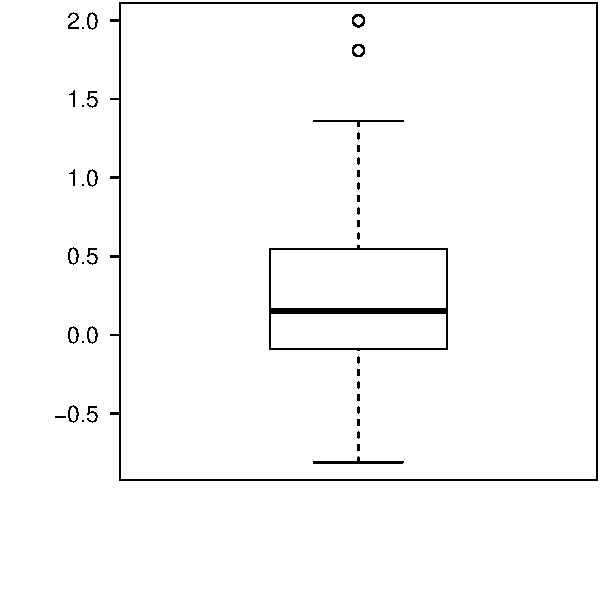
\includegraphics[width=.4\linewidth]{figures/plot-boring-plots-1} 
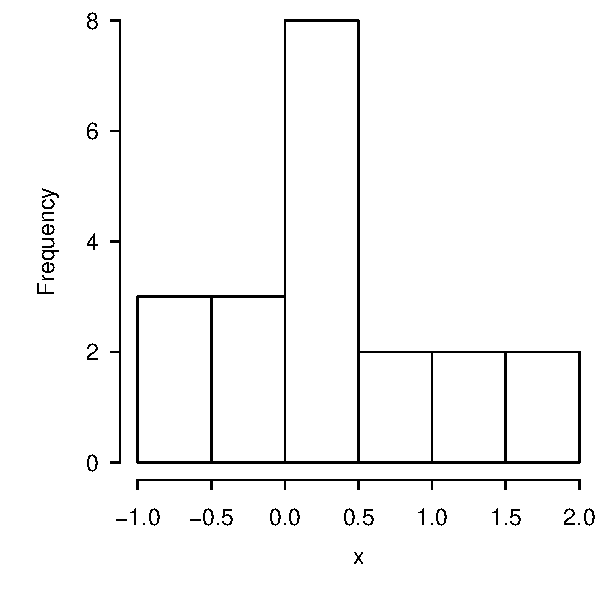
\includegraphics[width=.4\linewidth]{figures/plot-boring-plots-2} 

}



\end{knitrout}

Do the above chunks work? You should be able to compile the \TeX{}
The first element of \texttt{x} is 0.1449583. Boring boxplots
and histograms recorded by the PDF device:

\begin{knitrout}
\definecolor{shadecolor}{rgb}{0.969, 0.969, 0.969}\color{fgcolor}

{\centering 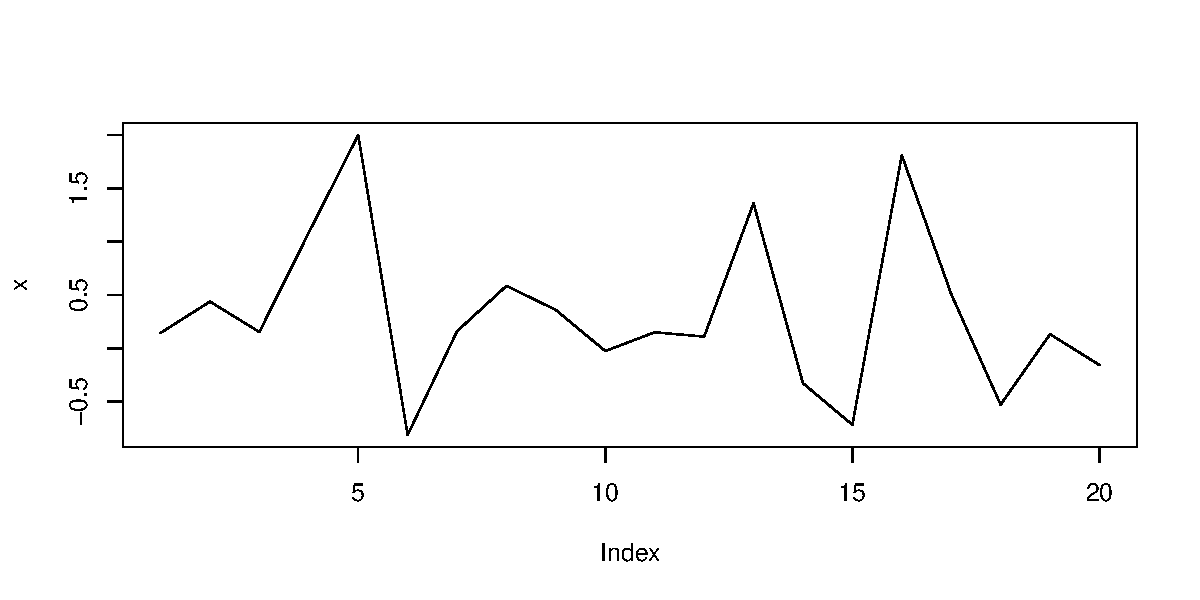
\includegraphics[width=.8\linewidth]{figures/plot-boring-plots2-1} 

}



\end{knitrout}

Do the above chunks work? You should be able to compile the \TeX{}

\end{document}
